\documentclass[floatfix,nofootinbib,superscriptaddress,fleqn]{revtex4-2}  
%\documentclass[aps,epsfig,tightlines,fleqn]{revtex4}
\usepackage[utf]{kotex}
\usepackage[HWP]{dhucs-interword}
\usepackage[dvips]{color}
\usepackage{graphicx}
\usepackage{bm}
%\usepackage{fancyhdr}
%\usepackage{dcolumn}
\usepackage{defcolor}
\usepackage{amsmath}
\usepackage{amsfonts}
\usepackage{amssymb}
\usepackage{amscd}
\usepackage{amsthm}
\usepackage[utf8]{inputenc}
 \usepackage{setspace}
%\pagestyle{fancy}

\begin{document}

\title{\Large 2022년 1학기 물리학 I: Quiz 18}
\author{김현철\footnote{Office: 5S-436D (면담시간 매주
    화요일-16:00$\sim$20:00)}} 
\email{hchkim@inha.ac.kr}
\author{Lee Hui-Jae} 
\email{hjlee6674@inha.edu}
\affiliation{Hadron Theory Group, Department of Physics,
Inha University, Incheon 22212, Republic of Korea }
\date{Spring semester, 2022}


\vspace{1.cm}

\maketitle

 
\noindent {\bf 문제 1. (40 pt)} 
불체가 좌우로 흔들리는 수평면에 놓여 있다. 수평면은 진동수 2.0 Hz로
단조화진동을 한다. 물체와 수평면 사이의 정지마찰계수는
0.50이다. 물체가 미끄러지지 않는 상태에서 단순조화진동의 최대진폭은
얼마인가? 
  
\noindent {\bf 풀이 : } 
물체가 미끄러지지 않고 수평면을 따라 단조화진동하기 위해 수평면이 물체에 주는 힘이
최대정지마찰력보다 작아야 한다. 수평면이 물체에 주는 힘을 $F$라 하면
\begin{align}
  F = ma  \leq f_s = \mu_s N = \mu_s mg
\end{align}
를 만족해야 한다. 다시쓰면
\begin{align}
  a  \leq \mu g
\end{align}
이다. 물체와 수평면은 단순조화진동을 하고 있으므로
 \begin{align}
   a = \frac{d^2x}{dt^2} = -\omega^2x,\,\,\,
   x = A\cos(\omega t+\phi)
 \end{align}
 이고 $\omega$는 각진동수로 진동수 $f$와 $\omega = 2\pi f$의 관계에 있다.
 따라서 조건을 다음과 같이 다시 쓸 수 있다.
 \begin{align}
   a = -(2\pi f)^2x = -(2\pi f)^2A\cos(\omega t+\phi)  \leq \mu g.
 \end{align}
 $-1\leq-\cos(\omega t+\phi)\leq 1$이므로 $(2\pi f)^2A \leq\mu g$이어야 하고
 최대진폭 $A$는
 \begin{align}
   A \leq \frac{\mu g}{4\pi^2f^2}
 \end{align}
 를 만족해야 물체가 미끄러지지 않고 단순조화진동한다. 최종적으로 최대진폭은
 \begin{align}
  \begin{split}
    A &= \frac{\mu g}{4\pi^2f^2} 
    = \frac{(0.50)(9.8\,\mathrm{m/s^2})}{4\pi^2(2.0\,\mathrm{Hz})^2}  \\
    &=0.031\,\mathrm{m}
  \end{split}
 \end{align}
 이다.
\newpage
 

\noindent {\bf 문제 2. (60 pt)}
그림~\ref{fig:1}처럼 질량이 $0.200$ kg인 물체 1이 마찰이 없는 윗면에서
8.00 m/s의 속력으로 오른쪽으로 미끄러지다가 정지한 물체 2와
탄성충돌을 한다. 물체 2와 연결된 용수철의 용수철 상수는
$1208.5\,\mathrm{N/m}$이다(용수철은 충돌에 영향을 주지 않는다고 가정하자).
충돌 후에 물체 2는 주기 0.10 초로 단순조화진동을 하고 물체 1은
윗면에서 아랫면으로 높이 $h=4.90$ m를 떨어졌다. 이때 물체 1이 착륙한
거리는 얼마인가? 
\begin{figure}[ht]
  \centering
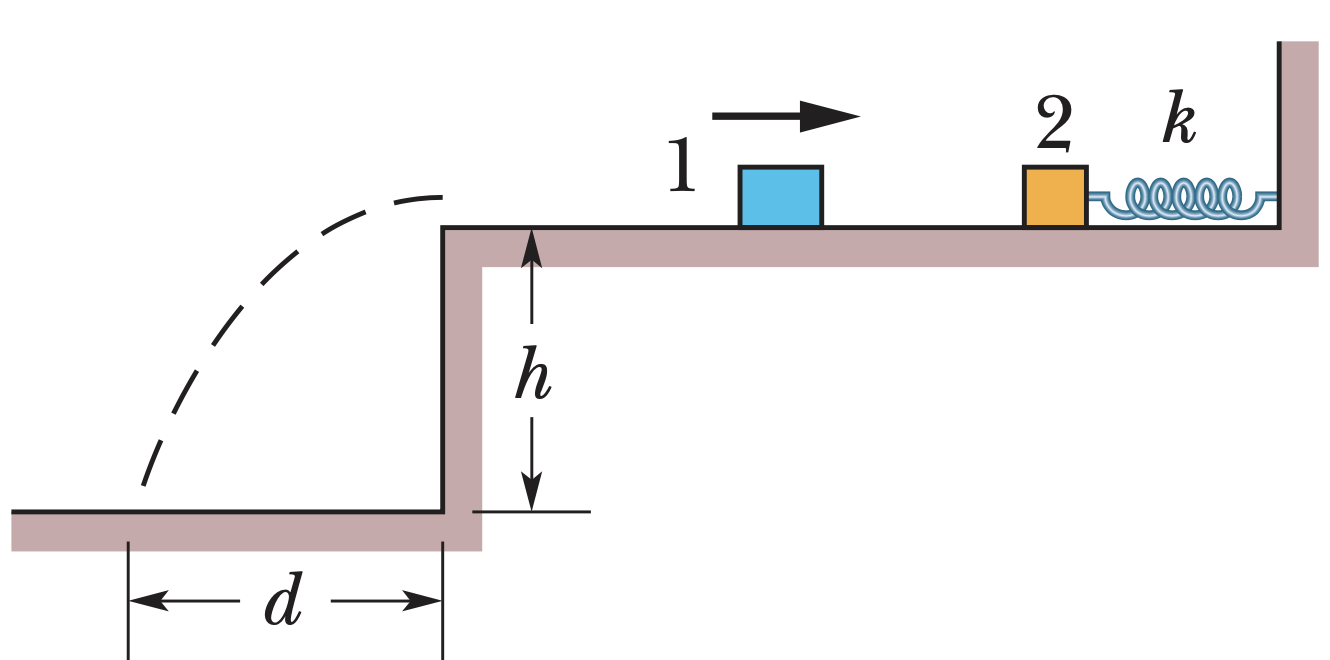
\includegraphics[scale=0.35]{Qfig18-1-20220511.png}
  \caption{문제 2}
  \label{fig:1}
\end{figure}

\noindent {\bf 풀이 : } 
처음 물체 1이 물체 2와 탄성 충돌하기 전에 용수철은 평형상태에 있었고 물체 2는
정지해있으므로 물체 1의 처음 속력을 $v_0$이라 하면 처음 역학적 에너지 $E_0$는
\begin{align}
  E_0 = \frac{1}{2}m_1v_0^2
\end{align}
이다. $m_1$은 물체 1의 질량이다. 물체 2와 탄성충돌하여 최대 변위까지 압축되었다가 
용수철의 평형점에서 물체 1과 물체 2가 분리된다. 물체 1은 평형점에서의 속력을 계속 가지고
움직이지만 물체 2는 용수철에 의해 평형점에서부터 속력이 줄어들기 때문이다. 
평형점에서 물체 1과 물체 2의 속력을 $v_1$이라 하면 역학적 에너지 보존법칙에 의해
\begin{align}\label{eq:2-1}
  E_0 = \frac{1}{2}(m_1+m_2)v_1^2
\end{align} 
라고 쓸 수 있다. $m_2$는 물체 2의 질량이다. 
물체 2의 운동에너지는 단순조화진동에 의해 용수철의
탄성 퍼텐셜에너지로 전환된다. 이 때 용수철의 최대 변위를 $A$라고 하면 
\begin{align}
  \frac{1}{2}m_2v_1^2 = \frac{1}{2}kA^2
\end{align}
이다. 물체 2가 진동하는 주기를 $T$라 하자. $T$는
\begin{align}
  T = \frac{2\pi}{\omega} = 2\pi\sqrt{\frac{m_2}{k}}
\end{align}
이므로 $m_2$는
\begin{align}
  m_2 =\frac{T^2k}{4\pi^2}
\end{align}
이고 식~\eqref{eq:2-1}은 다음과 같이 다시 쓸 수 있다.
\begin{align}\label{eq:2-2}
  \frac{1}{2}m_1v_0^2
  =\frac{1}{2}\left(m_1+\frac{T^2k}{4\pi^2}\right)v_1^2
  =\frac{1}{2}\left(\frac{4\pi^2m_1+T^2k}{4\pi^2}\right)v_1^2
\end{align}
이다. 물체 1이 $v_1$의 수평 속력을 가지고 아랫면으로 떨어지면 착륙한 거리 $d$는
\begin{align}
  d = v_1t,\,\,\,h=\frac{1}{2}gt^2\Longrightarrow d = v_1\sqrt{\frac{2h}{g}}
\end{align}
이다. 식~\eqref{eq:2-2}로부터 $v_1$은
\begin{align}
  v_1 = \sqrt{\frac{4\pi^2m_1}{4\pi^2m_1+T^2k}}v_0
\end{align}
이므로 $d$를 다시 쓸 수 있다.
\begin{align}
  d = \sqrt{\frac{8h\pi^2m_1}{g(4\pi^2m_1+T^2k)}}v_0.
\end{align}
수치를 넣어 $d$를 계산해보면 다음과 같다.
\begin{align}
  \begin{split}
    d &= \sqrt{\frac{8\pi^2(4.90\,\mathrm{m})(0.200\,\mathrm{kg})}
    {(9.80\,\mathrm{m/s^2})(4\pi^2(0.200\,\mathrm{kg})
    +(0.10\,\mathrm{s})^2(1208.5\,\mathrm{N/m}))}}(8.00\,\mathrm{m/s})  \\
    &= 5.0\,\mathrm{m}.
  \end{split}
\end{align}
물체 1이 착륙한 거리는 $5.0\,\mathrm{m}$이다.

\vspace{1.cm}
 
\noindent {\bf 문제 3. (60pt)  }
그림~\ref{fig:2}처럼 길이가 $L=1.85$ m인 막대가 물리진자로 진동한다.
\begin{figure}[ht]
  \centering
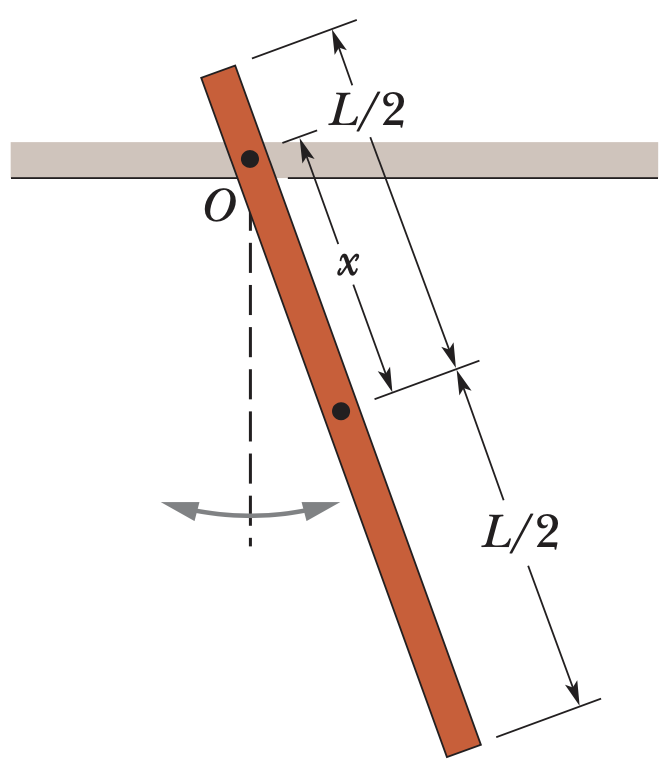
\includegraphics[scale=0.45]{Qfig18-2-20220511.png}
  \caption{문제 3}
  \label{fig:2}
\end{figure}
\begin{itemize}
\item[(가)] 막대의 중심질량과 회전축 사이의 거리 $x$가 얼마일 때
  주기가 최소이겠는가?
\item[(나)] 최소주기는 얼마인가?  
\end{itemize}
 
\noindent {\bf 풀이 : } 
\begin{itemize}
  \item[(가)] 물리진자가 진자운동하며 받는 돌림힘은 
  \begin{align}\label{eq:3-T}
    \tau = -(mg\sin\theta)x
  \end{align}
  이다. $x$는 회전축과 질량중심 사이 거리이고
   $\theta$는 막대의 평형축과 막대가 이루는 각도이다. $\theta$가 매우 작다고 가정하면
   \begin{align}
     \sin\theta \approx \theta
   \end{align}
로 근사할 수 있고 돌림힘에 대한 운동방정식을 다음과 같이 세울 수 있다.
\begin{align}
  I\frac{d^2\theta}{dt^2}=-mgx\theta.
\end{align}
이 경우 각진동수 $\omega$는
\begin{align}
  \omega = \sqrt{\frac{mgx}{I}}
\end{align}
이고 주기 $T$는
\begin{align}
  T = \frac{2\pi}{\omega}=2\pi \sqrt{\frac{I}{mgx}}
\end{align}
이다. 긴 막대의 경우 질량중심에서의 회전관성은 $\frac{1}{12}mL^2$이고 
평행축 정리를 이용하면 그림에 표현된 막대의 회전관성 $I$는 다음과 같다.
\begin{align}
  I = \frac{1}{12}mL^2 + mx^2.
\end{align}
따라서 막대의 주기 $T$는
\begin{align}\label{eq:3-T}
  T = 2\pi \sqrt{\left(\frac{L^2}{12gx} 
  + \frac{x}{g}\right)}
\end{align}
이다. 주기가 최소가 되는 $x$를 알기 위해 $T$를 $x$에 대해 미분해보자.
$T$를 $x$에 대해 미분한 값이 $0$이 되게 하는 $x$에서 $T$는 최소값을 가진다.
\begin{align}
  \frac{dT}{dx} = \pi \frac{-\frac{L^2}{12gx^2}+\frac{1}{g}}
  {\sqrt{\left(\frac{L^2}{12gx} + \frac{x}{g}\right)}}
  =\pi \left(\frac{12x^2-L^2}{12gx^2}\right)
  {\left(\sqrt{\frac{L^2}{12gx} + \frac{x}{g}}\right)}^{-1}.
\end{align}
위 식이 $0$이 되기 위해서 $12x^2-L^2=0$이어야 한다. 따라서 주기 $T$가
최소가 되도록 하는 $x$는
\begin{align}\label{eq:3-x}
  x = \sqrt{\frac{1}{12}}L = 0.534\,\mathrm{m}
\end{align}
이다.
  \item[(나)] 최소 주기 $T_{min}$은 식~\eqref{eq:3-T}에 식~\eqref{eq:3-x}을
  대입하여 얻는다. 최소 주기 $T_{min}$은
  \begin{align}
    T_{min} =  2\pi \sqrt{\left(\frac{L}{\sqrt{12}g} 
    + \frac{L}{\sqrt{12}g}\right)}
    =\frac{2\pi}{3^{1/4}}\sqrt{\frac{L}{g}}
  \end{align}
  이다. 수치를 대입하면
  \begin{align}
    \begin{split}
      T_{min} &= \frac{2\pi}{3^{1/4}}\sqrt{\frac{1.85\,\mathrm{m}}{9.80\,\mathrm{m/s^2}}} \\
      &=2.07\,\mathrm{s}
    \end{split}
  \end{align}
  로 최소주기는 $2.07\,\mathrm{s}$이다.
\end{itemize}  


\vspace{1.cm}
 

\noindent {\bf 문제 4. (60pt)}
그림~\ref{fig:3}처럼 질량이 $M=5.4$ kg인 물체가 마찰이 없는 탁자
위에서 용수철상수 $k=6\,000\,\mathrm{N/m}$인 용수철에 달린 채 벽에
부착되어 있다. 질량은 $m=95$ g이고 속도 $\vec{v}$의 크기가 630 m/s인
총알이 날아가 물체 박혔다. 총알이 박힐 때까지 용수철의 압축은 무시할
정도라고 가정하면 충돌 직후에
\begin{figure}[ht]
  \centering
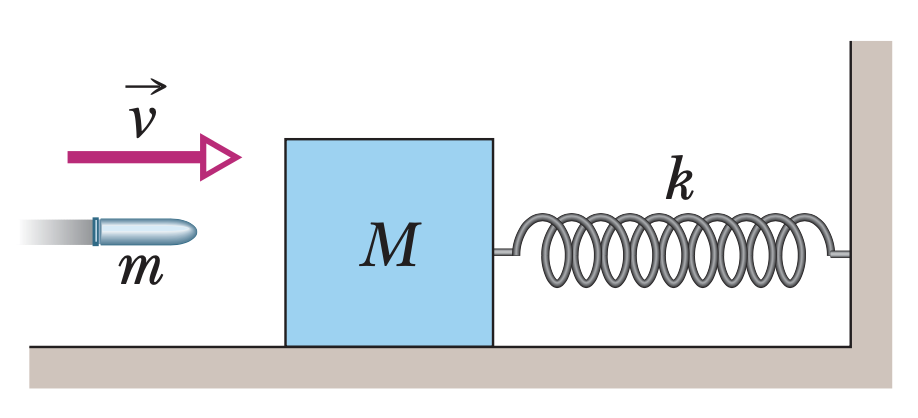
\includegraphics[scale=0.35]{Qfig18-3-20220511.png}
  \caption{문제 4}
  \label{fig:3}
\end{figure}
\begin{itemize}
\item[(가)] 물체의 속도와 
\item[(나)] 단순조화운동의 진폭은 각각 얼마인가?
\end{itemize}
 
\noindent {\bf 풀이 : } 
\begin{itemize}
  \item[(가)] 운동량 보존법칙을 통해 물체의 속도를 구해보자.
  총알의 질량을 $m$, 물체의 질량을 $M$라고 하고 처음 총알의 속력을 $v_0$,
  나중 총알과 물체의 속력을 $v_1$이라 하자. 운동량 보존법칙에 의해
  \begin{align}\label{eq:4-1}
    mv_0 = (m+M)v_1\Longrightarrow v_1 = \frac{m}{m+M}v_0
  \end{align}
  이다. 따라서 물체의 충돌 직후 속력은 
  \begin{align}
  \begin{split}
    v_1 &= \frac{(0.095\,\mathrm{kg})}
    {(0.095\,\mathrm{kg})+(5.4\,\mathrm{kg})}(630\,\mathrm{m/s})  \\
    &= 11\,\mathrm{m/s}
  \end{split}
  \end{align}
  이다. 따라서 물체의 속도의 크기는 $11\,\mathrm{m/s}$이다.
  \item[(나)] 역학적 에너지는 보존되므로 충돌한 직후 물체와 총알의 운동에너지의 합은 
  용수철이 최대변위에서 갖는 탄성 위치에너지와 같다. 최대변위를 $A$라고 하면
  \begin{align}
    \frac{1}{2}(m+M)v_1^2 = \frac{1}{2}kA^2
  \end{align}
  이다. $A$에 대해 정리하고 식~\eqref{eq:4-1}을 대입하면 최대변위 $A$는 다음과 같다.
  \begin{align}
    A = \sqrt{\frac{m+M}{k}}v_1 = \sqrt{\frac{m+M}{k}}\left(\frac{m}{m+M}\right)v_0
    =\frac{m}{\sqrt{k(m+M)}}v_0.
  \end{align}
  수치를 대입하여 구해보면
  \begin{align}
    \begin{split}
      A &= \frac{0.095\,\mathrm{kg}}{\sqrt{(6\,000\,\mathrm{N/m})((0.095\,\mathrm{kg})
      +(5.4\,\mathrm{kg}))}}(630\,\mathrm{m/s})  \\
      &= 0.33\,\mathrm{m}
    \end{split}
  \end{align}
  이므로 최대변위는 $ 0.33\,\mathrm{m}$이고 이는 곧 단순조화진동의 진폭이다.
\end{itemize}

 
\end{document}